\documentclass[tikz]{standalone}
\usepackage{pgfplots}
\pgfplotsset{compat=1.15}
\usepackage{mathrsfs}
\usetikzlibrary{arrows,calc}
\usepackage{tkz-euclide}

\pagestyle{empty}

\definecolor{AngleClr}{rgb}{0,0.39215686274509803,0}
\definecolor{ShapeClr}{rgb}{0.6,0.2,0}
\definecolor{BlueClr}{RGB}{13,93,184}
\definecolor{RedClr}{RGB}{204, 0, 0}

\begin{document}

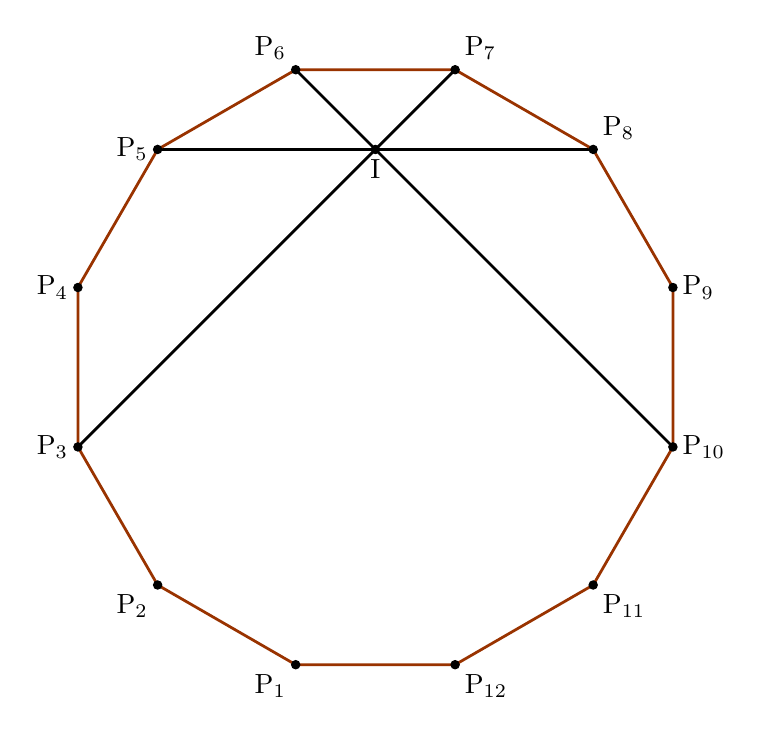
\begin{tikzpicture}[scale=.75]
\tkzSetUpLine[line width=1pt,color=black]
\tkzSetUpPoint[fill=black]

\tkzDefPoints{0/0/P0,2.7/0/P1}

\tkzDefRegPolygon[side,sides=12](P0,P1)

\tkzFillPolygon[fill=white](P1,P2,P3,P4,P5,P6,P7,P8,P9,P10,P11,P12)

\tkzDrawSegments[black,line width=1pt](P6,P9 P4,P8 P7,P11)

\tkzInterLL(P4,P8)(P7,P11) \tkzGetPoint{I}

\tkzDrawPolygon[color=ShapeClr](P1,P2,P3,P4,P5,P6,P7,P8,P9,P10,P11,P12)
\tkzDrawPoints[size=3](P1,P2,P3,P4,P5,P6,P7,P8,P9,P10,P11,P12,I)
\tkzLabelPoint[below left](P1){$\rm P_1$}
\tkzLabelPoint[below right](P2){$\rm P_{12}$}
\tkzLabelPoint[below right](P3){$\rm P_{11}$}
\tkzLabelPoint[right](P4){$\rm P_{10}$}
\tkzLabelPoint[right](P5){$\rm P_9$}
\tkzLabelPoint[above right](P6){$\rm P_8$}
\tkzLabelPoint[above right](P7){$\rm P_7$}
\tkzLabelPoint[above left](P8){$\rm \rm P_6$}
\tkzLabelPoint[left](P9){$\rm \rm P_5$}
\tkzLabelPoint[left](P10){$\rm P_4$}
\tkzLabelPoint[left](P11){$\rm P_3$}
\tkzLabelPoint[below left](P12){$\rm P_2$}

\tkzLabelPoint[below](I){$\rm I$}


\end{tikzpicture}

\end{document}
